\documentclass{bachelorthesis}

\newcommand{\ProjectTitle}{Semester Project: Intelligent Software Systems}
\newcommand{\ProjectSubtitle}{OPD-Vertex}
\newcommand{\ProjectFullName}{Outpatient Department Vertex}
\newcommand{\ApplicationName}{Med Flow}
\newcommand{\RunningReportTitle}{MED FLOW: OPD-VERTEX PROJECT REPORT}
\newcommand{\ProjectTagline}{A local-first consultation support system for recording, transcription, clinical draft generation, review, PDF export, and patient communication}
\newcommand{\GroupName}{Group 3}
\newcommand{\AuthorName}{Group 3}
\newcommand{\AuthorNames}{Gabriele Solazzo\\Aleksandra Kwiatkowska\\Gabija Staskeviciute\\Luigi Colluto\\Manish Raj Moriche\\Mats Haertel}
\newcommand{\SupervisorNames}{Devender Kumar and Riccardo Terrenzi}
\newcommand{\TeacherName}{Devender Kumar}
\newcommand{\TeacherEmail}{deku@mmmi.sdu.dk}
\newcommand{\SupervisorName}{Riccardo Terrenzi}
\newcommand{\SupervisorEmail}{rite@mmmi.sdu.dk}
\newcommand{\InstitutionName}{TEK Faculty -- S{\o}nderborg Campus}
\newcommand{\ProgrammeName}{Software Engineering, Semester 4}
\newcommand{\CourseId}{T630012401}
\newcommand{\SubmissionDate}{June 1st, 2026}
\newcommand{\RepositoryName}{Manish-SDU/OPD-VERTEX}
\usepackage{enumitem}
\usepackage[most]{tcolorbox}
\usepackage{tikz}
\usepackage{subcaption}

\usetikzlibrary{arrows.meta,positioning,fit,shapes.geometric}

\definecolor{VertexBlue}{HTML}{1D4ED8}
\definecolor{VertexTeal}{HTML}{0F766E}
\definecolor{VertexInk}{HTML}{0F172A}
\definecolor{VertexMuted}{HTML}{475569}
\definecolor{VertexLine}{HTML}{CBD5E1}
\definecolor{VertexPanel}{HTML}{F8FAFC}
\definecolor{VertexGreen}{HTML}{15803D}
\definecolor{VertexAmber}{HTML}{B45309}
\definecolor{VertexRed}{HTML}{B91C1C}

\hypersetup{
  colorlinks=true,
  linkcolor=black,
  urlcolor=black,
  citecolor=black,
  filecolor=black,
  pdftitle={\ProjectTitle},
  pdfauthor={\AuthorName}
}

\graphicspath{{assets/}{assets/charts/}}
\setlist[itemize]{leftmargin=1.4em,itemsep=0.25em,topsep=0.25em}
\setlist[enumerate]{leftmargin=1.6em,itemsep=0.25em,topsep=0.25em}
\renewcommand{\arraystretch}{1.2}
\setlength{\parindent}{0pt}
\setlength{\parskip}{0.55em}

\newtcolorbox{summarybox}{
  enhanced,
  colback=VertexPanel,
  colframe=VertexBlue,
  boxrule=0.7pt,
  arc=2mm,
  left=3mm,
  right=3mm,
  top=2mm,
  bottom=2mm
}

\newtcolorbox{calloutbox}[1]{
  enhanced,
  title=#1,
  colback=white,
  colframe=VertexTeal,
  coltitle=white,
  colbacktitle=VertexTeal,
  boxrule=0.7pt,
  arc=2mm,
  left=3mm,
  right=3mm,
  top=2mm,
  bottom=2mm
}

\newcommand{\optionalgraphic}[2][]{%
  \IfFileExists{#2}{%
    \includegraphics[#1]{#2}%
  }{%
    \fbox{\parbox{0.86\linewidth}{Missing figure: \texttt{\detokenize{#2}}. Copy the asset into the project before compiling.}}%
  }%
}

\newcommand{\metric}[2]{\textbf{#1}\hfill\textcolor{VertexMuted}{#2}}

\newcommand{\vertexcoverauthor}[1]{%
  \begin{minipage}[t]{0.31\textwidth}%
    \centering\scriptsize
    {\bfseries #1\par}%
    University of Southern Denmark\par
    Software Engineering\par
  \end{minipage}%
}

\makeatletter
\renewcommand{\maketitle}{%
  \pagenumbering{roman}%
  \begin{titlepage}%
    \thispagestyle{empty}%
    \centering
    \vspace*{0.45cm}%
    \rule{\textwidth}{0.7pt}\par
    \vspace{0.85em}%
    {\LARGE\scshape\MakeUppercase{\ProjectSubtitle}\par}%
    \vspace{0.85em}%
    \rule{\textwidth}{0.7pt}\par
    \vspace{1.35em}%
    {\small\scshape Semester Project 4\par}%
    \vspace{1.8em}%
    \noindent
    \vertexcoverauthor{Gabriele Solazzo}\hfill
    \vertexcoverauthor{Aleksandra Kwiatkowska}\hfill
    \vertexcoverauthor{Gabija Staskeviciute}\par
    \vspace{1.35em}%
    \noindent
    \vertexcoverauthor{Luigi Colluto}\hfill
    \vertexcoverauthor{Manish Raj Moriche}\hfill
    \vertexcoverauthor{Mats Haertel}\par
    \vspace{1.8em}%
    {\small\SubmissionDate\par}%
    \vspace{1.45em}%
    {\normalsize\bfseries\scshape Abstract\par}%
    \vspace{0.75em}%
    \begin{minipage}{0.86\textwidth}%
      \small\justifying
      \setlength{\parindent}{0pt}%
      \setlength{\parskip}{0pt}%
      \ProjectAbstractText

      \vspace{0.8em}%
      \noindent\textbf{\textit{Keywords}}\quad \ProjectKeywords
    \end{minipage}%
    \vfill
    \begin{minipage}{\textwidth}%
      \raggedright
      \rule{0.12\textwidth}{0.4pt}\par
      {\scriptsize $^{*}$ All authors contributed equally to this work.\par}%
    \end{minipage}%
  \end{titlepage}%
  \setcounter{footnote}{0}%
}
\makeatother
\newcommand{\ProjectAbstractText}{%
This report presents the design and implementation of Med Flow, a local-first consultation support system for outpatient departments. The application helps doctors manage appointment context, record consultations, transcribe spoken dialogue, generate AI-assisted clinical draft notes, review and edit the generated content, export approved reports as PDFs, and send follow-up communication to patients. The project includes a lightweight internal booking and scheduling module for the semester workflow, while treating scheduling as a replaceable boundary that can integrate with clinic or public-sector systems in production. Its architecture combines a FastAPI backend, persistence adapters, local speech transcription, prompt-driven report generation, review services, and an editable web interface. The implementation demonstrates the semester themes of artificial intelligence, component-based software, algorithms and data structures, and embedded-oriented design through privacy-aware processing, modular service boundaries, and explicit human approval before clinical information is finalized.%
}

\newcommand{\ProjectKeywords}{%
Artificial Intelligence \(\cdot\) Component-Based Systems \(\cdot\) Software Architecture \(\cdot\) Clinical Documentation \(\cdot\) Privacy-Aware Processing%
}

\title{\ProjectTitle\\\ProjectSubtitle}
\author{\GroupName\\[0.5em]\AuthorNames\\[1em]Teachers and supervisors\\\SupervisorNames}
\date{\InstitutionName\\\ProgrammeName\\Course ID: \CourseId\\\SubmissionDate}

\makeglossaries

\begin{document}

\maketitle
\tableofcontents

\mainmatter
\section{Introduction}

OPD-Vertex is a web-based platform for supporting outpatient medical consultations. The application helps doctors capture consultation audio, transcribe spoken dialogue, generate structured draft documentation, review the result, create PDFs, and send approved follow-up material to patients.

The project builds on the original OPD-Vertex proposal, which emphasized local processing, privacy-aware handling of medical data, and loosely coupled system design. The resulting system demonstrates how software can support documentation and communication in medical consultation settings while keeping sensitive data within the local environment.

\subsection{Motivation}

Medical consultations often require doctors to divide their attention between interacting with patients and documenting notes, prescriptions, and other relevant information. This can reduce consultation efficiency, increase the risk of missing important details, and delay the preparation of post-consultation documentation.

At the same time, the growing use of digital and AI-assisted healthcare tools raises concerns about privacy, legal compliance, protection of sensitive patient data, and dependence on external cloud services. OPD-Vertex is motivated by the need for a more efficient and privacy-conscious documentation workflow during medical consultations.

By supporting consultation recording, transcription, draft generation, and follow-up communication in a single system, the application aims to reduce administrative overhead while improving the quality and accessibility of consultation-related documentation. The project also explores how AI-assisted tools can support doctors without removing clinical responsibility from the final decision-making process.

\subsection{Objective}

The objective of this project is to design and implement a secure web-based consultation support system that assists doctors during and after medical consultations. The system records consultation audio, converts spoken dialogue into text, and generates a draft PDF containing consultation-related information and suggestions that the doctor can review, edit, approve, or decline before further processing.

Once approved by the doctor, the system supports continued handling of the consultation outcome by allowing relevant information, such as prescription details and follow-up material, to be sent to the patient by email. The system also provides functionality for viewing patient details, accessing doctor information, downloading generated PDF documents, and presenting relevant information through a dashboard.

\subsection{Delimitation}

The application is not intended to provide a complete medical administration system. It does not include full clinical record management, long-term clinical testing, user studies with external patients or healthcare providers, live medical deployment, advanced compliance certification, large-scale deployment, or full integration with existing healthcare systems.

The project focuses on supporting activities during and after an ongoing consultation. In the intended deployment context, healthcare providers are assumed to already rely on established scheduling systems. In line with the system's component-based architecture, scheduling is treated as an external concern that can be integrated through well-defined interfaces.

The generated transcription, summaries, suggestions, and PDF drafts are decision-support material for the doctor. They are not autonomous medical outputs. Final responsibility for reviewing, editing, approving, or declining generated content remains with the doctor before information is processed further or shared with the patient.
\section{Methodology}
\label{sec:methodology}

\subsection{Teamwork and Collaboration}
\label{subsec:teamwork-collaboration}

Tasks were distributed in pairs throughout most of the project, which supported collaboration and peer review. The workflow was organized in Trello across five completed sprints, keeping implementation, testing, diagram updates, and report work visible as the project evolved. \figref{fig:trello-board} shows the final sprint board used by the group.

\begin{figure}[htbp]
\centering
\optionalgraphic[width=\textwidth]{assets/img/Trello.png}
\caption{Final Trello sprint board used to coordinate implementation, testing, diagrams, and report tasks.}
\label{fig:trello-board}
\end{figure}
\FloatBarrier

During Sprint 1, the work centered on planning the project structure, preparing the project proposal, creating initial diagrams, and designing the database. Sprint 2 moved into setup and early implementation: configuring the application environment, drafting the first user interface, setting up SQL and NoSQL databases, and implementing authentication for patients, doctors, and administrators.

Sprint 3 added audio capture, speech-to-text transcription, the booking and scheduling flow, database fixes, and preparation for the midterm project presentation. Sprint 4 covered document versioning and editing, email sending, LLM-supported transcription, suggestions and report generation, UI completion, server-side PDF generation, logging, system testing, and AOP work. Sprint 5 focused on report completion, booking/admin permission refinements, database and diagram updates, PDF export naming, email attachments for generated PDFs, video recording, LaTeX report rewriting, and supervisor review. \appref{app:meeting-log} gives the detailed meeting log behind this sprint summary and maps each recorded meeting to the relevant sprint.

GitHub was used to share and manage the code in one shared repository\footnote{\url{\RepositoryUrl}}, keeping contributions organized while supporting collaboration. The group met around twice per week to review progress, coordinate tasks, and resolve blockers. WhatsApp handled daily updates, while Discord was used for sharing files, data, and other project resources.

\subsection{Scope Context and Source Selection}
\label{subsec:scope-context-source-selection}

During early scoping, the project was narrowed around clinical documentation rather than general medical administration, image analysis, or unrelated laboratory AI. This direction is supported by studies showing that physicians spend a large amount of time on electronic records and clerical work during and after consultations\refcite{1,2,3}. The team therefore selected a problem where software engineering could address a concrete workflow: capturing consultation audio, converting it to text, generating a draft note, and supporting a structured review step.

The Danish context also shaped the scope. The Danish digital health strategy describes a healthcare system that should feel coherent and trustworthy for patients while making daily workflows easier for healthcare professionals\refcite{7}. At SDU and Odense University Hospital, CAI-X presents clinical AI as a collaboration between healthcare staff, researchers, and engineers, with solutions chosen from the needs and challenges clinicians face in daily work\refcite{8}. This gave the project a useful local reference point for treating AI as workflow support instead of as a replacement for clinical judgement.

The most directly related Danish example found during source selection is CAI-X's AID\_NOTE project\refcite{9}, which evaluates Ambient Scribe speech-to-text solutions across clinical settings and measures documentation quality, time consumption, user experience, and economic impact. Med Flow is not a deployment of that project, but it addresses a comparable type of problem at semester-project scale. The technical source selection therefore focused on risk guidance for AI medical scribes\refcite{4}, robust local speech recognition\refcite{10}, and responsible AI governance\refcite{11,12}.

\subsection{Application of Course Knowledge}
\label{subsec:course-knowledge}

\begin{itemize}
	\item \textbf{Artificial Intelligence:} Faster-Whisper converts consultation audio into text, while the local Qwen3:8b model generates structured report drafts, prescription suggestions, and Suggestive Mode alerts. The AI work is tied to explicit safeguards: prompt grounding, JSON-schema validation, hallucination checks, ASR artifact filtering, and doctor approval before clinical output becomes final.
	\item \textbf{Component-Based Systems:} FastAPI routers, application services, domain contracts, repositories, and infrastructure adapters separate authentication, patients, appointments, consultations, transcription, review, prescriptions, PDF, email, and audit. This makes it possible to replace Whisper, Ollama, persistence adapters, email delivery, or booking integration without rewriting the whole workflow.
	\item \textbf{Operating Systems:} Docker Compose was used to containerize the FastAPI application, Whisper sidecar, MySQL, MongoDB, MailHog, and supporting services. This connected the operating-systems course knowledge to the project through process isolation, port mapping, filesystem volumes, environment variables, and reproducible local deployment across different developer machines.
	\item \textbf{Algorithms and Data Structures:} the system uses status transitions for consultations and appointments, transcript chunk assembly, patient and appointment filtering, version-history lists for edited documents, deterministic safety rules for prescriptions, and structured JSON objects validated before they enter the review flow. These structures turn raw speech and model output into data that can be searched, reviewed, tested, and rendered as PDFs.
	\item \textbf{Designing Software Systems with Embedded Elements:} although the application is not deployed on a microcontroller, it follows embedded-oriented constraints by running AI services locally, budgeting memory and VRAM, validating CPU/GPU fallback paths, containerizing services with Docker Compose, and avoiding cloud APIs for sensitive processing. The hardware envelope shows that the design is constrained by real local machines rather than unlimited server resources.
	\item \textbf{Data Management:} MySQL stores users, patients, appointments, consultations, prescriptions, and audit logs as structured records, while MongoDB stores transcripts, generated documents, prompts, email templates, and AI artifacts. The split supports relational consistency for approved clinical data and schema flexibility for iterative AI outputs.
\end{itemize}
\section{Problem Analysis}

\subsection{Risks and Limitations of Manual Documentation}

A large-scale descriptive study analysing approximately 100 million patient encounters with about 155 thousand physicians found that the average time spent on Electronic Health Records (EHR) is about 16 minutes per encounter. When contrasted with a typical 15 to 20 minute patient consultation, this indicates that administrative work can take almost as much time as the medical evaluation itself.

The American Medical Association has also highlighted that administrative tasks can occupy a large part of a standard shift. This forces doctors to multitask by actively listening while typing summaries. Divided focus increases the risk of documentation errors and missed diagnostic verbal cues.

To reduce these bottlenecks, the system should capture information passively through audio rather than relying entirely on manual input. The automation must function as a decision-support tool by generating editable drafts and real-time suggestions while ensuring that the doctor keeps final clinical responsibility and oversight.

\subsection{Security and Privacy in AI-Assisted Healthcare}

According to Article 9 of the General Data Protection Regulation (GDPR), medical data such as clinical notes, transcriptions, and prescriptions is classified as a special category of personal data. This classification significantly restricts how it can be collected, stored, and processed.

Many AI documentation tools rely on transmitting data to external cloud servers, which creates concerns around data sovereignty and purpose limitation. Cloud dependency also introduces operational vulnerability if the external network fails.

To reduce the risk of data leaks and internet dependency, OPD-Vertex is designed as a locally hosted system using open-source LLMs deployed on the clinic's internal network. This architecture aims to keep audio processing, transcription, and document generation local, ensuring that sensitive data remains private and under the clinic's control.

\subsection{Architectural Challenges}

Traditional EHR systems are often built as monolithic or tightly coupled structures. This creates a major problem because updating a single feature can require modifying and risking the stability of the entire system. This becomes especially challenging when working with AI and speech-to-text components, which evolve quickly and need to be replaceable independently.

The system also handles diverse data types: live audio metadata, raw speech-to-text transcriptions, generated reports, user authentication, patient records, prescriptions, and audit logs. User and patient records require relational consistency, while transcripts and AI-generated artifacts require schema flexibility.

Forcing these conflicting data types into one database model can create performance and maintainability problems. The system must therefore balance strict relational consistency for user administration and patient records with dynamic schema flexibility for AI data processing.

\subsection{Problem Statement}

Modern medical documentation tools place a heavy administrative burden on doctors, yet many cloud-based AI automation tools introduce data privacy risks and operational vulnerabilities. Traditional monolithic architectures and strict database structures are also poorly suited to the rapid evolution of local AI tools and the combination of structured and unstructured clinical datasets.

This project therefore seeks to answer the following question:

\begin{summarybox}
How can a software system be designed and implemented to automate medical consultation documentation using local AI assistance, while ensuring data privacy, security, and architectural flexibility?
\end{summarybox}
\section{Requirements}
\label{sec:requirements}

The requirements were organized with a MoSCoW-style priority structure. Must-have requirements define the minimum useful consultation-support system. Should-have and could-have requirements describe important improvements and possible extensions. Will-not-have requirements clarify the boundaries of the implementation.

Their implementation and validation evidence is traced in Section~\ref{subsec:requirements-coverage}, where each requirement is linked to the report sections and appendices that demonstrate it.

\subsection{Actors and Use Cases}
\label{subsec:actors-use-cases}

This subsection defines the system actors and the required user goals. The design chapter reuses these actors as inputs instead of redefining them, so role responsibilities and use cases remain traceable from one place.

The implemented workflow is centered on three roles: doctors, administrators, and patients. Doctors own the consultation and approval flow, patients can book appointments and read their own consultation and prescription information, and administrators manage configuration that affects AI prompts and email templates. All three roles use the same email/password login screen. Staff and patient passwords are stored as bcrypt hashes, and the current implementation does not include doctor-generated password setup links, magic-login links, or patient login URLs sent by doctors. The doctor email workflow sends approved follow-up material with a PDF attachment rather than an authentication link. Table~\ref{tab:primary-use-cases} summarizes the primary implemented use cases used later as design inputs.

\begin{figure}[htbp]
\centering
\resizebox{\textwidth}{!}{%
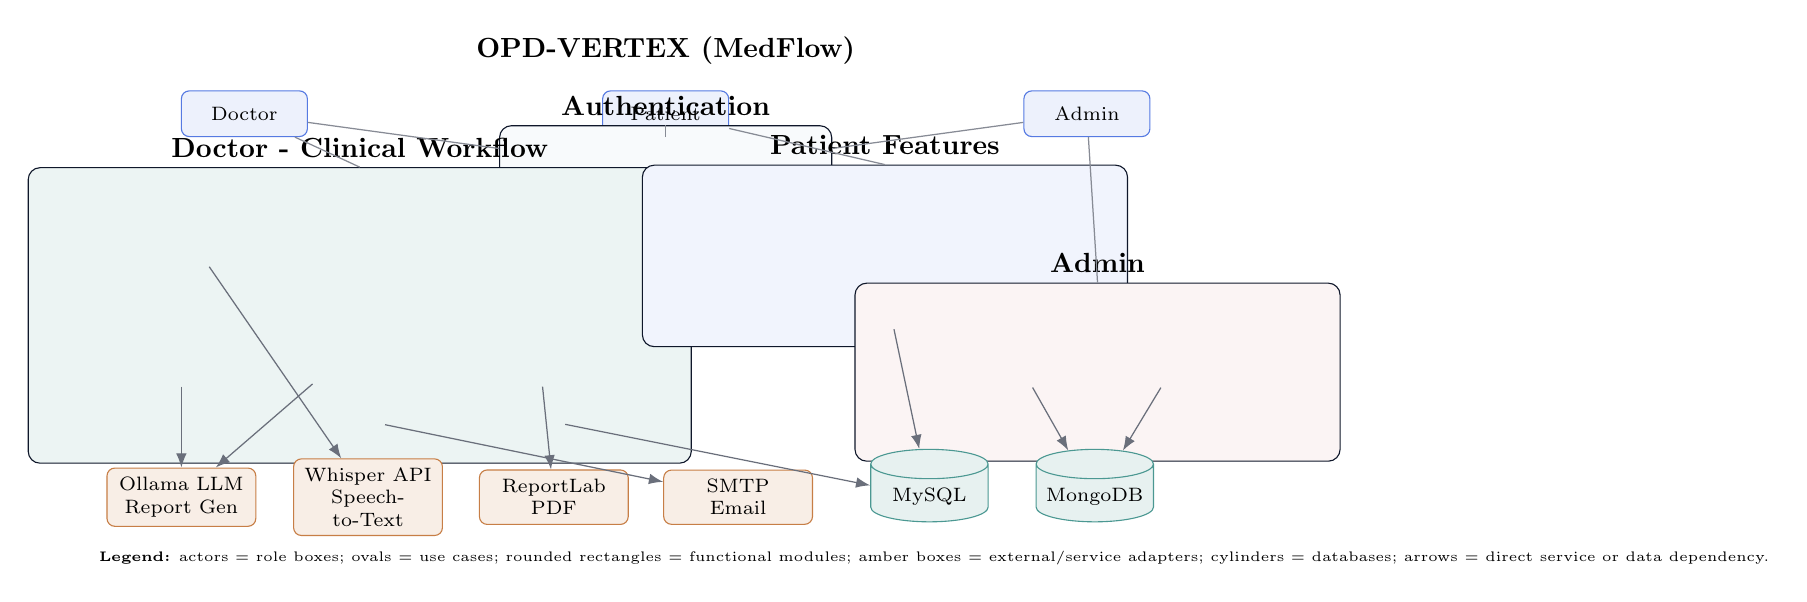
\begin{tikzpicture}[
	font=\scriptsize,
	actor/.style={draw=VertexBlue!75, fill=VertexBlue!8, rounded corners=1mm, align=center, minimum width=1.6cm, minimum height=0.58cm},
	usecase/.style={draw=VertexBlue!55, fill=white, ellipse, align=center, text width=2.15cm, minimum height=0.58cm, inner sep=1.4mm},
	authbox/.style={draw=VertexInk, fill=VertexPanel, rounded corners=1.5mm, inner sep=2.2mm},
	doctorbox/.style={draw=VertexInk, fill=VertexTeal!8, rounded corners=1.5mm, inner sep=2.2mm},
	patientbox/.style={draw=VertexInk, fill=VertexBlue!6, rounded corners=1.5mm, inner sep=2.2mm},
	adminbox/.style={draw=VertexInk, fill=VertexRed!5, rounded corners=1.5mm, inner sep=2.2mm},
	service/.style={draw=VertexAmber!75, fill=VertexAmber!10, rounded corners=1mm, align=center, text width=1.65cm, minimum height=0.62cm, inner sep=1.2mm},
	data/.style={draw=VertexTeal!75, fill=VertexTeal!10, cylinder, shape border rotate=90, aspect=0.25, align=center, text width=1.25cm, minimum height=0.68cm, inner sep=1.2mm},
	link/.style={-{Latex[length=1.8mm]}, draw=VertexInk!62, line width=0.45pt},
	assoc/.style={draw=VertexInk!50, line width=0.45pt}
]
\node[font=\bfseries] at (0,5.15) {OPD-VERTEX (MedFlow)};

\node[actor] (doctor) at (-5.35,4.35) {Doctor};
\node[actor] (patient) at (0,4.35) {Patient};
\node[actor] (admin) at (5.35,4.35) {Admin};

\node[usecase, text width=1.25cm] (login) at (-0.80,3.62) {Log In};
\node[usecase, text width=1.25cm] (logout) at (0.80,3.62) {Log Out};
\node[authbox, fit=(login)(logout), label={[font=\bfseries]above:Authentication}] (auth) {};

\node[usecase] (record) at (-6.15,2.92) {Record \& Transcribe Audio};
\node[usecase] (create) at (-3.88,2.92) {Create Consultation};
\node[usecase] (browse) at (-1.62,2.92) {Browse \& Search Patients};
\node[usecase] (viewconsult) at (-6.15,2.18) {View Consultations};
\node[usecase] (review) at (-3.88,2.18) {Review Draft Notes};
\node[usecase] (approve) at (-1.62,2.18) {Approve / Reject Draft};
\node[usecase] (report) at (-6.15,1.44) {Generate Clinical Report};
\node[usecase] (suggest) at (-3.88,1.44) {Suggestive Safety Review};
\node[usecase] (pdf) at (-1.62,1.44) {Generate Prescription PDF};
\node[usecase] (email) at (-5.02,0.70) {Email Prescription};
\node[usecase] (appt) at (-2.75,0.70) {View/Create/Accept Appointments};
\node[doctorbox, fit=(record)(create)(browse)(viewconsult)(review)(approve)(report)(suggest)(pdf)(email)(appt), label={[font=\bfseries]above:Doctor - Clinical Workflow}] (doctorflow) {};

\node[usecase] (profile) at (1.65,2.92) {View Own Profile};
\node[usecase] (ownrx) at (3.92,2.92) {View Own Prescriptions};
\node[usecase] (ownappt) at (2.78,2.18) {View/Create/Delete Appointments};
\node[patientbox, fit=(profile)(ownrx)(ownappt), label={[font=\bfseries]above:Patient Features}] (patientfeatures) {};

\node[usecase] (prompts) at (4.35,1.42) {Manage Prompt Templates};
\node[usecase] (templates) at (6.62,1.42) {Manage Email Templates};
\node[usecase] (health) at (5.48,0.68) {View System Health};
\node[adminbox, fit=(prompts)(templates)(health), label={[font=\bfseries]above:Admin}] (adminfeatures) {};

\node[service] (ollama) at (-6.15,-0.52) {Ollama LLM\\Report Gen};
\node[service] (whisper) at (-3.78,-0.52) {Whisper API\\Speech-to-Text};
\node[service] (reportlab) at (-1.42,-0.52) {ReportLab\\PDF};
\node[service] (smtp) at (0.92,-0.52) {SMTP\\Email};
\node[data] (mysql) at (3.35,-0.52) {MySQL};
\node[data] (mongo) at (5.45,-0.52) {MongoDB};

\draw[assoc] (doctor) -- (auth);
\draw[assoc] (patient) -- (auth);
\draw[assoc] (admin) -- (auth);
\draw[assoc] (doctor) -- (doctorflow.north);
\draw[assoc] (patient) -- (patientfeatures.north);
\draw[assoc] (admin) -- (adminfeatures.north);
\draw[link] (record) -- (whisper);
\draw[link] (report) -- (ollama);
\draw[link] (suggest) -- (ollama);
\draw[link] (pdf) -- (reportlab);
\draw[link] (email) -- (smtp);
\draw[link] (appt) -- (mysql);
\draw[link] (ownappt) -- (mysql);
\draw[link] (prompts) -- (mongo);
\draw[link] (templates) -- (mongo);

\node[anchor=north west, align=left, font=\tiny] at (-7.32,-1.08) {\textbf{Legend:} actors = role boxes; ovals = use cases; rounded rectangles = functional modules; amber boxes = external/service adapters; cylinders = databases; arrows = direct service or data dependency.};
\end{tikzpicture}%
}
\caption{Implemented Med Flow use-case view for doctors, patients, administrators, infrastructure components, and external services.}
\label{fig:use-case-diagram}
\end{figure}
\FloatBarrier

\begin{table}[htbp]
\centering
\small
\begin{tabularx}{\textwidth}{@{}P{0.10\textwidth}P{0.16\textwidth}YP{0.30\textwidth}@{}}
\TableTopRule
\rowcolor{VertexTableBlue}
\VertexTableHead{ID} & \VertexTableHead{Actor} & \VertexTableHead{Goal} & \VertexTableHead{Primary flow} \\
\TableMidRule
\rowcolor{VertexTableStripe}
UC-1 & All roles & Authenticate and reach the correct dashboard. & User enters email and password, receives a JWT cookie, and is routed to the role-aware dashboard. \\
UC-2 & Patient & Book an appointment. & Patient selects appointment details for themselves, submits reason and time, and creates appointment context. \\
\rowcolor{VertexTableStripe}
UC-3 & Doctor / Admin & Manage appointment status. & Doctor or administrator confirms, cancels, or marks no-show appointments; only doctors start consultations. \\
UC-4 & Doctor & Record and transcribe a consultation. & Doctor starts the linked consultation, records audio, receives transcript updates, and finalizes transcription. \\
\rowcolor{VertexTableStripe}
UC-5 & Doctor & Generate AI-supported clinical material. & Doctor sends transcript and patient context through local AI services to create report, prescription, and alert drafts. \\
UC-6 & Doctor & Review and edit generated drafts. & Doctor reads transcript, structured report, prescription draft, and suggestive alerts, then edits Markdown if needed. \\
\rowcolor{VertexTableStripe}
UC-7 & Doctor & Approve, export, and send final records. & Doctor approves or rejects drafts, downloads the PDF, and can send approved follow-up email with attachment. \\
UC-8 & Doctor & Search patient history. & Doctor searches patients, opens a patient detail page, and reviews consultation and prescription history. \\
\rowcolor{VertexTableStripe}
UC-9 & Patient & View own clinical information. & Patient logs in with email/password and sees only their own appointments, consultations, and prescriptions. \\
UC-10 & Administrator & Maintain configurable content and auditability. & Administrator edits prompts and email templates and reviews audit entries for those changes. \\
\TableBottomRule
\end{tabularx}
\caption{Primary Med Flow use cases by actor.}
\label{tab:primary-use-cases}
\end{table}
\FloatBarrier

\subsection{Must-Have Requirements}
\label{subsec:must-have-requirements}

\begingroup
\small
\begin{longtable}{@{}P{0.16\textwidth}P{0.76\textwidth}@{}}
\caption{Must-have requirements.}\\
\TableTopRule
\rowcolor{VertexTableBlue}
\VertexTableHead{ID} & \VertexTableHead{Requirement} \\
\TableMidRule
\rowcolor{VertexTableStripe}
F-1 & The system must manage a doctor consultation queue, including consultation context created from booking or scheduling. \\
F-2 & The system must capture consultation audio locally. \\
\rowcolor{VertexTableStripe}
F-3 & The system must transcribe speech to text locally. \\
F-4 & The system must generate a doctor-editable structured clinical note from the transcript and patient context, including presenting problem, relevant history, assessment, treatment or medication plan, follow-up, and patient instructions when supported by the consultation. \\
\rowcolor{VertexTableStripe}
F-5 & The system must generate a doctor-editable prescription draft with medication name, dosage, frequency, duration, patient instructions, and review alerts for missing dosage information or possible allergy/contraindication conflicts. \\
F-6 & The system must allow doctors to edit, approve, or reject generated clinical notes and prescription drafts before they become final records. \\
\rowcolor{VertexTableStripe}
F-7 & The system must generate downloadable PDFs from approved clinical report and prescription data. \\
F-8 & The system must send approved patient follow-up or prescription summaries by configured email and prevent unapproved drafts from being emailed. \\
\rowcolor{VertexTableStripe}
NF-1 & Privacy: all AI processing must be performed locally. \\
NF-2 & Security: the system must use authentication and role-based access for doctors, administrators, and patients, with patients restricted to their own records. \\
\rowcolor{VertexTableStripe}
NF-3 & Data protection: the system must hash stored passwords and be designed for encrypted deployment channels and storage. \\
NF-4 & Modularity: components must be loosely coupled and replaceable. \\
\rowcolor{VertexTableStripe}
NF-5 & Reliability: the system must persist consultation state, transcripts, generated documents, and prescription versions so interrupted workflows can be retried without losing approved data. \\
NF-6 & Auditability: the system must preserve traceability for important actions and edits, including prompt updates, email-template updates, doctor report edits with version history, and review approval or rejection status changes. \\
\TableBottomRule
\end{longtable}
\endgroup

\subsection{Should-Have Requirements}
\label{subsec:should-have-requirements}

\begingroup
\small
\begin{longtable}{@{}P{0.16\textwidth}P{0.76\textwidth}@{}}
\caption{Should-have requirements.}\\
\TableTopRule
\rowcolor{VertexTableBlue}
\VertexTableHead{ID} & \VertexTableHead{Requirement} \\
\TableMidRule
\rowcolor{VertexTableStripe}
F-9 & The system should display a live transcript during consultation. \\
F-10 & The system should allow doctors to view past consultations. \\
\rowcolor{VertexTableStripe}
F-12 & The system should keep booking and scheduling replaceable, so an external clinic or public-sector booking service can create consultation context through stable interfaces. \\
NF-7 & Usability: the interface should be user-friendly and efficient. \\
NF-8 & Performance: on the target machine, local transcription should operate with RTF $\leq 1.0$. For a typical consultation transcript, the system should generate structured notes, prescription draft, and clinical alerts within $\leq 40$ seconds on recommended hardware and within $\leq 120$ seconds on minimum hardware. \\
\TableBottomRule
\end{longtable}
\endgroup

\subsection{Could-Have Requirements}
\label{subsec:could-have-requirements}

\begingroup
\small
\begin{longtable}{@{}P{0.16\textwidth}P{0.76\textwidth}@{}}
\caption{Could-have requirements.}\\
\TableTopRule
\rowcolor{VertexTableBlue}
\VertexTableHead{ID} & \VertexTableHead{Requirement} \\
\TableMidRule
\rowcolor{VertexTableStripe}
F-11 & The system could support multiple doctors for sharing documents, such as a shareable report sent to a doctor other than the family doctor. \\
NF-9 & The system could allow administrators to configure how long consultation data, transcripts, and prescriptions are stored, and must support secure deletion of expired records. \\
\TableBottomRule
\end{longtable}
\endgroup

\subsection{Will-Not-Have Requirements}
\label{subsec:will-not-have-requirements}

\begingroup
\small
\begin{longtable}{@{}P{0.16\textwidth}P{0.76\textwidth}@{}}
\caption{Will-not-have requirements.}\\
\TableTopRule
\rowcolor{VertexTableBlue}
\VertexTableHead{ID} & \VertexTableHead{Requirement} \\
\TableMidRule
\rowcolor{VertexTableStripe}
NF-10 & The system will not use cloud-based AI services. \\
NF-11 & The system alone, excluding the doctor, is not enough for diagnosis. \\
\TableBottomRule
\end{longtable}
\endgroup

\section{Design}

This chapter describes the design of Med Flow, focusing on the principles used to structure the system, the main components and their interactions, the data model, and the cross-cutting concerns of the application.

\subsection{Design Goals and Principles}

Med Flow was designed as a privacy-first, locally hosted clinical assistant for outpatient departments. Five principles guided the design decisions:

\begin{itemize}
  \item \textbf{Local-first execution:} sensitive processing runs inside the clinic environment, so no consultation data is sent to a third-party cloud LLM.
  \item \textbf{Component-based design:} the system is split into bounded modules, each with its own application service and domain contracts.
  \item \textbf{Loose coupling through ports and adapters:} external dependencies are exposed as domain ports and implemented by adapters, so application logic does not depend on concrete libraries.
  \item \textbf{Replaceability of AI components:} transcription, LLM generation, and suggestive review are independent ports, allowing them to be swapped without changing core application logic.
  \item \textbf{Human-in-the-loop approval:} no AI output is written to the relational database without doctor approval.
\end{itemize}

These principles keep the system maintainable through a layered architecture and make it easier to extend because each component can be replaced without rewriting the core.

\subsection{System Overview and Architecture}

Before writing code, the team sketched the main user journeys and screen layouts in Figma. The mockups were intentionally lightweight because UI design was not the main focus. They were used to agree on the doctor login, doctor dashboard, consultation page with audio recording, draft review page, and patient view. The three implemented user roles were doctor, administrator, and patient. The review page evolved during development and was split into view, editor, and print modes after the team decided to support Markdown editing.

\begin{figure}[htbp]
\centering
\fbox{%
  \begin{minipage}{0.86\linewidth}
  \centering
  Insert Figma mockup screenshot for doctor dashboard and consultation screens.
  \end{minipage}%
}
\caption{Initial Figma mockup of the doctor dashboard and consultation screens.}
\end{figure}

The target architecture is a set of cooperating services organized around the clinical workflow: identity, patient, consultation, transcription, LLM orchestration, suggestive review, PDF generation, notification, and audit. Public endpoints sit behind an API gateway, while AI components run on dedicated local services. Each service owns its own datastore to preserve loose coupling.

In the implemented system, this design is realized on a smaller scale. The logical components live as Python modules inside a single FastAPI application. The transcription module runs as a separate Whisper sidecar, the LLM runs in Ollama, MySQL stores relational data, and MongoDB stores AI documents. All services are packaged as Docker containers and orchestrated with Docker Compose, giving the project a reproducible setup and a clear migration path toward the target architecture.

\subsection{Component-Based System Design}

The system was decomposed into loosely coupled components. Each component has a single responsibility and can be developed, tested, or replaced independently. In the current implementation, many of these components live as modules inside the local backend app, while the diagram represents the logical boundaries that the architecture is intended to support.

\begin{figure}[htbp]
\centering
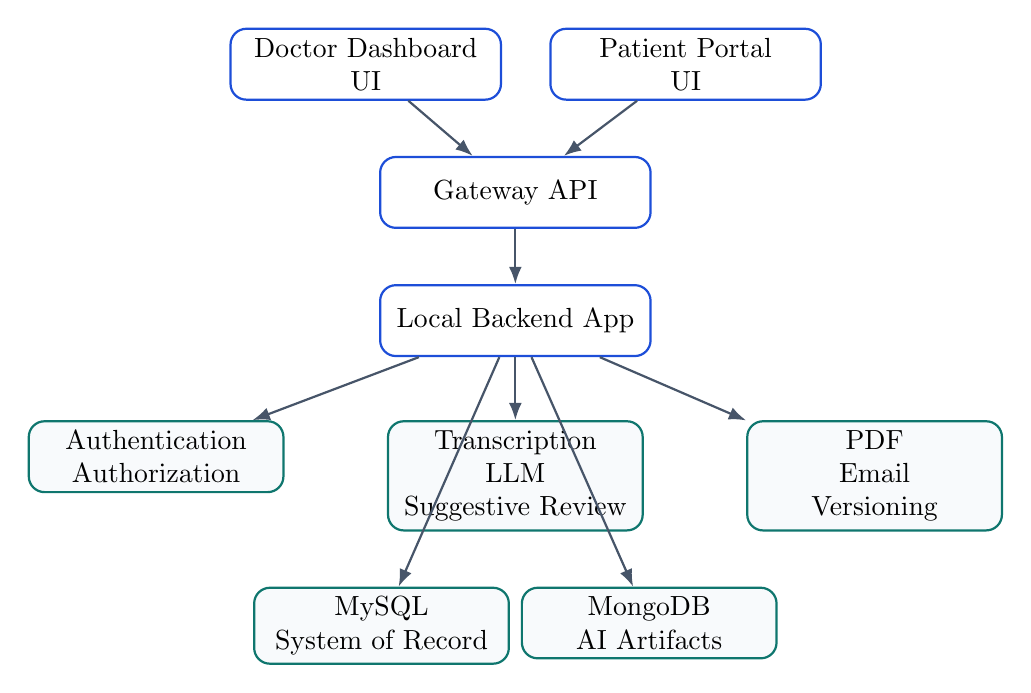
\begin{tikzpicture}[
  component/.style={rectangle,rounded corners=2mm,draw=VertexBlue,fill=white,thick,align=center,text width=3.2cm,minimum height=0.9cm},
  adapter/.style={rectangle,rounded corners=2mm,draw=VertexTeal,fill=VertexPanel,thick,align=center,text width=3cm,minimum height=0.8cm},
  arrow/.style={-{Latex[length=2.2mm]},draw=VertexMuted,thick}
]
\node[component] (doctor) {Doctor Dashboard\\UI};
\node[component,right=0.6cm of doctor] (patient) {Patient Portal\\UI};
\node[component,below=0.7cm of doctor,xshift=1.9cm] (gateway) {Gateway API};
\node[component,below=0.7cm of gateway] (backend) {Local Backend App};
\node[adapter,below left=0.8cm and 1.2cm of backend] (auth) {Authentication\\Authorization};
\node[adapter,below=0.8cm of backend] (ai) {Transcription\\LLM\\Suggestive Review};
\node[adapter,below right=0.8cm and 1.2cm of backend] (doc) {PDF\\Email\\Versioning};
\node[adapter,below=0.7cm of ai,xshift=-1.7cm] (mysql) {MySQL\\System of Record};
\node[adapter,below=0.7cm of ai,xshift=1.7cm] (mongo) {MongoDB\\AI Artifacts};
\draw[arrow] (doctor) -- (gateway);
\draw[arrow] (patient) -- (gateway);
\draw[arrow] (gateway) -- (backend);
\draw[arrow] (backend) -- (auth);
\draw[arrow] (backend) -- (ai);
\draw[arrow] (backend) -- (doc);
\draw[arrow] (backend) -- (mysql);
\draw[arrow] (backend) -- (mongo);
\end{tikzpicture}
\caption{Logical component diagram showing Med Flow components and interfaces.}
\end{figure}

On the user-facing side, the Doctor Dashboard is the main interface for doctors and gives access to the patient list, consultation recording, draft review, and prescription approval. The Patient Portal is used by patients to log in and read their own consultations and prescriptions. Both interfaces are server-rendered with Jinja2 templates and communicate with the backend through the Gateway API.

Authentication and authorization validate credentials, issue JWT tokens, and enforce role-based access control. The Email Notification Service sends patient summaries through SMTP. The Document Editing and Versioning service manages generated report lifecycle, Markdown edits, and version history so every revision made by a doctor can be traced.

The AI pipeline starts with local audio capture, which sends consultation audio to the Faster-Whisper transcription module. The LLM Orchestrator manages prompts, retries, and structured output validation. Generation is delegated to the local LLM runtime through Ollama or vLLM, and ReportLab renders approved Markdown reports into printable PDFs.

\subsection{Aspect-Oriented Programming for Cross-Cutting Concerns}

Logging, performance measurement, error capture, and request tracing touch almost every layer of the system, but they do not belong to the business logic of any single module. To avoid scattering logging statements throughout the codebase, these concerns are handled with an Aspect-Oriented Programming approach.

The AOP layer is based on a class-level decorator that automatically wraps every public method of a class with entry, exit, and error logging while measuring wall-clock duration. Middleware logs every HTTP request, including method, path, client IP, status code, and duration, without changing route handlers.

This keeps application services and repository classes free of observability boilerplate while producing uniform log entries with consistent duration units. A future migration to tracing or metrics infrastructure would require changing one focused area instead of refactoring the entire codebase.

\subsection{Data Design and Dual-Database Architecture}

Med Flow uses a dual-database design to separate the system of record from iterative AI artifacts. The relational store provides consistency for clinically meaningful data, while the document store provides flexibility for evolving AI outputs.

\begin{table}[htbp]
\centering
\begin{tabularx}{\textwidth}{@{}>{\raggedright\arraybackslash}p{0.22\textwidth}>{\raggedright\arraybackslash}X@{}}
\toprule
\textbf{Database} & \textbf{Responsibility} \\
\midrule
MySQL 8.4 & Stores staff, patients, consultations, approved prescriptions, and audit logs. It acts as the structured system of record. \\
MongoDB 7 & Stores consultation documents, generated documents, prescription artifacts, LLM prompts, and email templates. It acts as the flexible document store for AI artifacts. \\
Shared linkage & The \texttt{consultation\_id} connects relational records to document records across the two stores. \\
\bottomrule
\end{tabularx}
\caption{Dual-database ownership model.}
\end{table}

MySQL stores doctors and administrators with roles, hashed passwords, license data, and specialization; patients with demographics, allergies, medical history, and hashed passwords; consultations with status transitions from recording to transcribing, processing, review, approved, rejected, or cancelled; prescriptions with versioning; and append-only audit logs.

MongoDB stores semi-structured artifacts from the AI pipeline: transcripts and working notes, drafted reports, suggestive reviews, generated PDFs, versioned prompt templates, and editable patient communication templates. The iterative and fast-changing artifacts remain in MongoDB, while the legally meaningful approved prescription is moved into MySQL only after doctor approval.

\begin{figure}[htbp]
\centering
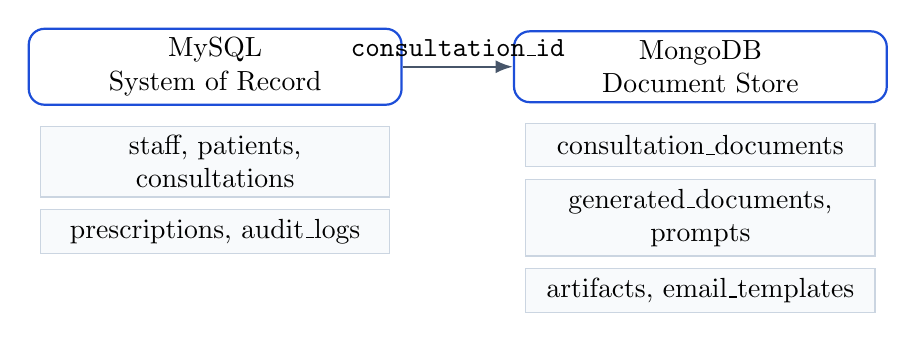
\begin{tikzpicture}[
  store/.style={rectangle,rounded corners=2mm,draw=VertexBlue,fill=white,thick,align=center,text width=4.5cm,minimum height=0.9cm},
  item/.style={rectangle,draw=VertexLine,fill=VertexPanel,align=center,text width=4.2cm,minimum height=0.55cm},
  arrow/.style={-{Latex[length=2.2mm]},draw=VertexMuted,thick}
]
\node[store] (mysql) {MySQL\\System of Record};
\node[item,below=0.25cm of mysql] (staff) {staff, patients, consultations};
\node[item,below=0.15cm of staff] (presc) {prescriptions, audit\_logs};
\node[store,right=1.4cm of mysql] (mongo) {MongoDB\\Document Store};
\node[item,below=0.25cm of mongo] (docs) {consultation\_documents};
\node[item,below=0.15cm of docs] (gen) {generated\_documents, prompts};
\node[item,below=0.15cm of gen] (email) {artifacts, email\_templates};
\draw[arrow] (mysql) -- node[above]{\texttt{consultation\_id}} (mongo);
\end{tikzpicture}
\caption{Relational schema and document collections connected by consultation identity.}
\end{figure}

\subsection{Main Workflow and AI Pipeline}

The consultation flow is implemented as three smaller workflows: consultation creation, AI processing, and prescription approval. The doctor opens the patient list, selects a patient, and starts a consultation. The system creates a new record with status \texttt{recording}; audio is captured in the browser and streamed to the backend through a WebSocket, which forwards chunks to the Whisper sidecar in near real time. Partial transcripts are stored so the session can survive a disconnect. When the doctor stops recording, the consultation moves to \texttt{processing} and the AI pipeline starts.

The AI pipeline contains two LLM calls followed by a safety pass. The transcript normalizer converts the raw transcript into structured JSON and filters speech artifacts. The clinical-note generator combines the normalized transcript with patient context, including age, allergies, and medical history, and asks Qwen3:8b to produce a structured object containing diagnosis, medications, instructions, follow-up date, lab tests, imaging, and a Markdown rendering of the full report.

Suggestive Mode then performs a second pass. An LLM-based clinical safety review is merged with deterministic rule-based checks, such as missing dose, frequency, duration, allergy conflicts, and contraindication conflicts. The combined output is shown to the doctor as advisory alerts. Nothing is written to the prescription unless the doctor accepts it during editing.

\begin{figure}[htbp]
\centering
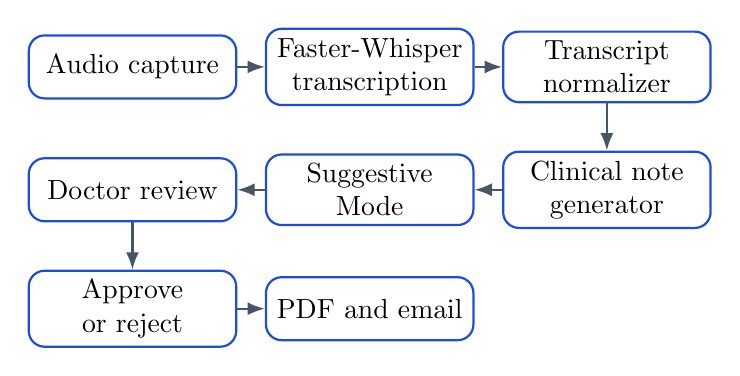
\begin{tikzpicture}[
  stage/.style={rectangle,rounded corners=2mm,draw=VertexBlue,fill=white,thick,align=center,text width=2.4cm,minimum height=0.8cm},
  arrow/.style={-{Latex[length=2.2mm]},draw=VertexMuted,thick}
]
\node[stage] (audio) {Audio capture};
\node[stage,right=0.35cm of audio] (asr) {Faster-Whisper transcription};
\node[stage,right=0.35cm of asr] (normalizer) {Transcript normalizer};
\node[stage,below=0.6cm of normalizer] (llm) {Clinical note generator};
\node[stage,left=0.35cm of llm] (suggest) {Suggestive Mode};
\node[stage,left=0.35cm of suggest] (review) {Doctor review};
\node[stage,below=0.6cm of review] (approve) {Approve or reject};
\node[stage,right=0.35cm of approve] (pdf) {PDF and email};
\draw[arrow] (audio) -- (asr);
\draw[arrow] (asr) -- (normalizer);
\draw[arrow] (normalizer) -- (llm);
\draw[arrow] (llm) -- (suggest);
\draw[arrow] (suggest) -- (review);
\draw[arrow] (review) -- (approve);
\draw[arrow] (approve) -- (pdf);
\end{tikzpicture}
\caption{End-to-end consultation workflow from audio capture to approved output.}
\end{figure}

After generation, the doctor opens the review page, optionally edits the Markdown report, and either approves or rejects the draft. If approved, the system builds a prescription, saves it in MySQL with \texttt{is\_approved = true} and the next version number, marks the generated document as approved, and updates the consultation status. After approval, the doctor can download the PDF and send a plain-text summary email to the patient.

\subsection{Privacy, Security and Error Handling}

The design treats clinical data as information that must not leave the local environment. Speech-to-text and LLM services run locally, so there is no path that sends transcripts or reports to a remote provider. Login is handled with bcrypt password hashing and short-lived JWT tokens stored in an HTTP-only cookie. Role-based access control protects routes that mutate clinical content, and patients can see only their own consultations and prescriptions.

The audit log records significant actions, including user, role, action, target, IP address, timestamp, and JSON details. Administrative changes to prompts and templates are also audited. The manual approval gate ensures that no AI output is written into the relational prescriptions table without explicit doctor approval, and email gating ensures that patient summaries are sent only after approval.

Error handling follows a small predictable model. Domain-level problems raise a \texttt{ValueError}, which the API translates into 400 or 404 responses. Unexpected failures become 500 responses. Transcription errors leave the consultation in its current state so the doctor can retry. LLM errors are caught by validation and drafts are left unchanged. PDF and email failures return 500 without altering the underlying record.

The implementation does not claim full regulatory compliance. TLS termination, stronger authorization tests, and at-rest encryption are treated as future deployment requirements.

\subsection{UI Overview}

The UI is intentionally simple and task-focused. Each screen serves one role and one job, and every page shares a common base layout and CSS bundle. The doctor dashboard is the role-aware home page for clinicians. The consultation page hosts live recording and transcription. The review page is the core human-in-the-loop screen because it shows the AI draft, structured fields, suggestive-mode alerts, Markdown editor, and approve, reject, print, and email actions.

The patient portal is read-only with respect to clinical data. The admin configuration view lets administrators edit prompts and email templates while maintaining an audit trail.

\subsection{Scope Decisions and Future Enhancements}

The project specification mentioned a patient booking system, but after discussion with the supervisor the team decided not to build an in-house scheduler. Clinics usually already have scheduling solutions, often connected to national identity and e-health infrastructure. Duplicating this functionality would not add much value to the system.

The component-based architecture makes it possible to defer scheduling cleanly. Patients and consultations are independent modules with stable contracts, so an external scheduler can pre-create consultations through the same APIs. Doctors currently create consultations directly from the patient list, and the AI pipeline works end-to-end from there.

Future enhancements include a queued retry layer for transient Whisper or Ollama failures, hardened deployment security, expanded Suggestive Mode rules with a broader interaction database, and a booking component with patient-facing calendar, slot management, and reminders.
\section{Implementation}

This chapter outlines the implementation approach for Med Flow. It covers the development process, core components, and technologies used. The system follows a component-based architecture with a FastAPI backend, MySQL and MongoDB databases, Faster-Whisper for transcription, Ollama or vLLM for clinical summarization, ReportLab for PDF generation, and SMTP for email delivery. The application is containerized with Docker for consistent deployment across environments. Configuration and logging are managed with Pydantic and the project's logging infrastructure.

\subsection{API Layer and Routing}

The API layer is built using FastAPI. It defines and serves HTTP endpoints and acts as the main entry point for user interactions.

The main API gateway is defined in \texttt{router.py}. This file creates the central API router and includes sub-routers for each domain, such as authentication, patients, consultations, transcriptions, review, prescriptions, PDF, email, audit, and administration. Each sub-router is responsible for a specific set of endpoints, which keeps the system separated by concern and easier to extend.

FastAPI dependency injection is used to manage authentication, database sessions, and shared resources. Dependencies are defined in \texttt{deps.py} and injected into endpoint functions. Each domain has its own router module where endpoints are defined as functions using decorators such as \texttt{@router.get} and \texttt{@router.post}.

\subsection{Authentication and Authorization}

Authentication ensures secure access control using role-based authorization. The system uses FastAPI dependency injection, JWT tokens, and a modular service structure.

The main authentication logic is implemented in \texttt{AuthApplicationService}, which bridges the API layer and domain logic. Domain models represent users, login requests, and the authentication interface, creating a consistent contract between application and infrastructure layers.

\begin{itemize}
  \item \textbf{User:} represents a system user with roles.
  \item \textbf{LoginRequest:} encapsulates login credentials.
  \item \textbf{AuthService:} defines an abstract interface for authentication logic and allows alternative implementations.
\end{itemize}

After successful authentication, the system assigns a JWT to the user. The token is used for later authenticated requests and includes user identity and role. Authentication checks are enforced through FastAPI dependencies that validate JWTs from incoming requests and ensure that only authenticated users can reach protected endpoints.

\subsection{Transcription Module}

The transcription component enables live conversion of audio into text, which can then be processed into clinical documentation. It is designed to be scalable, replaceable, and integrated with the other components.

The workflow is orchestrated by \texttt{TranscriptionApplicationService}, which handles streaming audio data, temporary audio and text chunks, and finalization of the complete transcription. The actual speech-to-text conversion is handled by Faster-Whisper through a dedicated adapter. The adapter communicates with a local Whisper microservice using HTTP.

\begin{enumerate}
  \item \textbf{Session initialization:} temporary storage is created for incoming audio data through \texttt{start\_transcription\_session}.
  \item \textbf{Audio streaming and chunk handling:} audio is streamed to the backend. The service processes chunks and sends them to the Faster-Whisper API for transcription. Partial results are stored using the temporary transcript chunk repository.
  \item \textbf{Transcript assembly:} temporary chunks are assembled into the final transcription, which is then stored in MongoDB as a consultation document.
  \item \textbf{Error handling:} the module handles network interruptions, partial uploads, and API errors. Temporary storage ensures that progress is not lost if a session is interrupted.
\end{enumerate}

\subsection{LLM Orchestration}

The LLM orchestration component enables clinical note creation, report generation, and suggestions using the locally integrated Ollama model. The core logic lives in LLM client and adapter classes, such as \texttt{ollama\_client.py} and \texttt{ollama\_adapter.py}. These classes provide an interface for sending prompts, receiving completions, validating structured output, and handling model health checks.

The \texttt{OllamaClient} handles HTTP communication with the local Ollama or vLLM runtime. Application services or endpoints use predefined prompt templates stored in the prompt directory. These templates are populated with clinical context, patient data, transcript content, and other inputs before being sent to the model runtime.

The orchestration workflow is:

\begin{enumerate}
  \item \textbf{Prompt construction:} templates are populated with patient context and consultation content.
  \item \textbf{Request dispatch:} the prompt is sent through \texttt{OllamaClient}, which handles retries, timeouts, and errors.
  \item \textbf{Response handling:} the response is returned to the calling service and can be displayed directly or processed further by Suggestive Mode.
  \item \textbf{Error handling:} network errors, model unavailability, and malformed responses are handled by the orchestration layer to provide informative errors.
\end{enumerate}

\subsection{PDF Generation}

The PDF generation module creates structured PDF documents from clinical data produced by consultations and prescriptions. This feature is important for shareable and printable records.

PDF generation is implemented with ReportLab. An adapter class encapsulates formatting and creation logic, while the service orchestrates data retrieval, PDF creation, and storage. The workflow starts with collecting consultation, patient, staff, and prescription data from repositories. The \texttt{ReportLabPdfGenerator} then formats the data into a document with page layouts, styles, tables, and visual elements. The resulting file is stored and made available for download or email attachment after approval.

\subsection{Email Notification Service}

The email notification service sends emails to patients containing consultation summaries and prescription information. It supports communication between the application and its users after doctor approval.

Email sending is handled by \texttt{SmtpEmailService}. It constructs and sends emails using the SMTP library \texttt{smtplib}. The service supports plain text and HTML emails, as well as attachments such as PDF files. Multipart messages are built with Python's \texttt{email.mime} package.

During development, MailHog was used as the SMTP server. MailHog captures outgoing emails so developers can view and verify email content without sending real messages. The email workflow constructs an email message, connects to the SMTP server, sends the email, and then allows developers to inspect the captured message through MailHog's web interface.

\subsection{Database Integration}

The system uses a dual-database architecture to manage structured and unstructured data. MySQL is used for structured data such as user accounts, patient records, consultations, prescriptions, and audit logs. MongoDB is used for semi-structured data such as clinical documents, consultation transcripts, generated reports, and finalized AI artifacts.

SQLAlchemy manages the MySQL connection and session lifecycle. Reusable database access is provided through functions such as \texttt{get\_engine()} and \texttt{get\_session()}. PyMongo manages MongoDB connections, with \texttt{get\_database()} returning the database handle used by document repositories.

Both databases are abstracted behind repository classes. Application services interact with repositories rather than directly with database clients. This pattern improves separation of concerns, testability, and maintainability.
\section{Validation}

\subsection{Validation Strategy}

The validation process follows a five-tier test pyramid. Unit tests exercise pure domain logic and the in-memory adapter layer. Integration tests drive FastAPI routes through Starlette's \texttt{TestClient} with a deterministic LLM mock, so HTTP behavior, validation, and persistence wiring are covered without external services. Smoke tests boot the full ASGI application and assert that critical-path endpoints, including login, dashboard, consultation list, and health checks, return successful responses.

Stress tests apply concurrent and sustained load to the in-memory repositories to surface ID collisions, race conditions, and memory growth. Benchmark tests measure per-operation latency. Two non-functional risks receive dedicated suites: LLM hallucination resistance and ASR artifact suppression. Both run hermetically against mocks in CI and can re-run live against a CUDA GPU when the local Ollama daemon and Whisper service are reachable.

\subsection{Test Inventory and Outcome}

The most recent suite execution reported in the source report ran 326 automated tests in 18.0 seconds, yielding a 100.0\% pass rate with 326 passed, 0 failed, and 0 skipped. Live-service tests gate themselves on the availability of Ollama or the Whisper microservice. On a developer workstation with both running, the live tier also passes.

\begin{table}[htbp]
\centering
\begin{tabularx}{\textwidth}{@{}>{\raggedright\arraybackslash}p{0.24\textwidth}>{\raggedright\arraybackslash}X@{}}
\toprule
\textbf{Tier} & \textbf{Coverage focus} \\
\midrule
Unit & Pure domain logic, entities, services, and in-memory adapters. \\
Integration & FastAPI routes, request validation, persistence wiring, and deterministic LLM behavior. \\
Smoke & Application boot and critical-path HTTP endpoint availability. \\
Stress & Concurrent writes, repeated mutations, list invariants, ID uniqueness, and memory growth. \\
Benchmark & p50, p95, and p99 latency for hot application paths. \\
Specialized AI/ASR & Hallucination resistance, structured output validation, ASR artifact suppression, and isolation checks. \\
Manual UI & Cookie lifecycle, downloads, CSS rendering, speaker turns, layout responsiveness, and release checklist validation. \\
\bottomrule
\end{tabularx}
\caption{Automated and manual validation tiers.}
\end{table}

\begin{figure}[htbp]
\centering
\begin{subfigure}{0.48\textwidth}
  \centering
  \optionalgraphic[width=\linewidth]{assets/charts/pass_rate.png}
  \caption{Pass rate}
\end{subfigure}\hfill
\begin{subfigure}{0.48\textwidth}
  \centering
  \optionalgraphic[width=\linewidth]{assets/charts/test_distribution.png}
  \caption{Test distribution}
\end{subfigure}
\caption{Validation overview charts.}
\end{figure}

\subsection{LLM Hallucination Resistance}

Every LLM-backed component runs on open-source weights served locally by Ollama. The reference model is Qwen3:8b under the Apache 2.0 license. No proprietary cloud APIs are used, which keeps patient data on-premises and makes validation reproducible without a billing account.

Three failure classes are explicitly guarded:

\begin{enumerate}
  \item \textbf{Structural hallucinations:} malformed JSON, missing required keys, or a literal \texttt{None} rendered into a clinical field are caught by Pydantic validation in \texttt{OllamaClient.generate\_json}. The client retries once and then raises an error.
  \item \textbf{Content hallucinations:} invented allergies, diagnoses, or medications absent from the transcript are guarded by prompt-level grounding instructions and a post-generation contradiction check enforced in \texttt{test\_llm\_hallucination.py}.
  \item \textbf{Cross-consultation leakage:} text from a previous patient surfacing in the current note is prevented by stateless per-call prompts and verified by isolation tests that interleave generations from two synthetic patients.
\end{enumerate}

\texttt{test\_real\_llm.py} re-asserts the same invariants against the live Ollama daemon and falls back gracefully to the mock when the daemon is unreachable.

\begin{figure}[htbp]
\centering
\optionalgraphic[width=0.72\textwidth]{assets/charts/hallucination_matrix.png}
\caption{Hallucination guard matrix.}
\end{figure}

\subsection{ASR Robustness}

Faster-Whisper is tuned for clinical dictation with beam size 5, temperature 0, and the setting \path{condition_on_previous_text=False}. This reduces the decoder's tendency to echo earlier captions on silent or noisy audio. A WebRTC VAD at level 3 strips silence before the encoder, so the model does not receive empty buffers.

The Faster-Whisper hallucination test suite asserts four invariants: silence results in an empty transcript, known artifact strings such as ``Thanks for watching!'' and ``[Music]'' are dropped, word error rate stays below 0.15 on a synthetic clinical fixture, and two concurrent sessions never share partial-transcript state.

\subsection{Open-Source Model Selection}

Six open-source models served by Ollama were ranked on four criteria: JSON-schema adherence, hallucination rate, end-to-end note latency at p95, and peak VRAM footprint. All candidates were quantized to \texttt{Q4\_K\_M} to fit the 8 GB VRAM envelope, evaluated on $n = 30$ synthetic consultations, and run at temperature 0.2.

Qwen3:8b was selected because it achieved 100\% JSON validity and zero hallucinations within the 8 GB VRAM budget. Phi3:medium was more accurate but exceeded the budget, while the 4B models traded too much accuracy for speed. The choice is not hard-wired: the deployed model is read from \texttt{OLLAMA\_MODEL}, and \texttt{test\_real\_llm.py} re-validates whichever model Ollama is currently serving.

\begin{figure}[htbp]
\centering
\optionalgraphic[width=0.78\textwidth]{assets/charts/model_comparison.png}
\caption{Model comparison on the Med Flow prompt set.}
\end{figure}

\subsection{Hardware Constraints and Deployment Envelope}

The application was tested across the team's personal laptops to confirm that it runs on realistic consumer hardware rather than a single tuned reference machine. The tested devices included a Microsoft Surface Pro 11 with Snapdragon X Plus and 16 GB unified memory, a MINISFORUM UM890 Pro mini-PC with 32 GB DDR5 memory, an ASUS Vivobook 15 F1504VA with Intel Core 7 150U and 16 GB RAM, and an Apple MacBook Air 13-inch with 16 GB unified memory.

None of these devices has a discrete GPU, so the model stack is sized for a shared-memory profile. Whisper large-v3 in int8 uses approximately 3.0 GB and runs on CPU or NPU through \texttt{compute\_type=int8}. Qwen3:8b is served by Ollama at \texttt{Q4\_K\_M}, using approximately 6.1 GB peak memory, which fits within the 16 GB envelope of every device.

Latency varies by host, and the Surface and MacBook are roughly three to four times slower than a CUDA workstation. The application remains usable end-to-end. Reference latency numbers were collected separately on a CUDA workstation with an RTX 4060 Laptop GPU and 8 GB VRAM.

\subsection{Performance Benchmarking}

The benchmark suite uses Python's \texttt{time.perf\_counter} to time 10 hot paths over 100 to 500 iterations each, recording p50, p95, and p99 latency. Each measurement has an explicit upper-bound assertion so a regression fails the build instead of silently degrading performance.

\begin{figure}[htbp]
\centering
\optionalgraphic[width=0.82\textwidth]{assets/charts/benchmark_latency.png}
\caption{p50, p95, and p99 latency for benchmarked operations against in-memory adapters.}
\end{figure}

The results are favorable: every operation finishes in well under a millisecond at the 99th percentile. This indicates that the application layer is not the bottleneck. Production latency will be higher because real MySQL and MongoDB adapters add network and disk I/O, but the benchmark establishes that the domain logic imposes negligible overhead.

\subsection{Stress and Concurrency}

Stress testing verifies that the in-memory layer behaves correctly under load beyond what a single clinic shift would normally generate. Three scenarios run: 1,000 sequential patient creations to check for ID collisions and unbounded memory growth, 500 list-after-mutation invariant checks to confirm repository snapshots remain consistent, and concurrent consultation creation through \texttt{ThreadPoolExecutor} to expose race conditions in the create/list path.

All scenarios complete within their wall-clock budgets and assert post-conditions on count, uniqueness, and ordering.

\subsection{Manual UI Validation}

Browser-level concerns that are awkward to automate with the current toolchain are covered by a 10-case manual checklist executed before each release. These concerns include cookie lifecycle, file downloads, CSS rendering of speaker turns, and layout responsiveness.

Each case is recorded with a unique identifier from TC001 to TC010, the scenario under test, reproduction steps, expected result, observed result, and status. At the time of writing, every case is passing. Future work proposes replacing this checklist with a Playwright end-to-end suite once the test infrastructure stabilizes.

\subsection{Threats to Validity}

Three threats temper the conclusions drawn from the validation results. First, benchmark figures use in-memory adapters, so production latency on MySQL and MongoDB will be higher. These numbers should be read as a lower bound that proves the domain code is not the bottleneck, not as production service-level objectives.

Second, live LLM tests are opportunistic. When Ollama is unavailable, they fall back to a deterministic mock and are reported as passing. A green CI run alone therefore does not prove that the live model still satisfies the hallucination guards; the live tier must be re-run on a developer workstation before each release.

Third, the WER fixture is synthetic. The published Faster-Whisper large-v3 envelope is used as ground truth for accuracy claims, and a real annotated clinical corpus is the most important validation improvement.

\subsection{Future Validation Work}

Future validation work includes WER measurement on a real annotated clinical corpus, mutation testing with \texttt{mutmut} on the domain core, property-based testing with \texttt{hypothesis} on status transitions, Playwright end-to-end tests replacing the manual UI checklist, and JMeter-based load testing for the deployed HTTP API.
\section{Discussion}
\label{sec:discussion}

\subsection{Scope and Outcome}
\label{subsec:discussion-scope-outcome}

Med Flow demonstrates the consultation-support path promised by the project scope: a doctor can work with patient information, start a consultation, capture audio, obtain a transcript, generate structured clinical material, review and edit the AI output, approve the result, export a PDF, and send follow-up communication. The result is strongest as a workflow prototype with a real implementation behind it, not only as a design proposal.

The most important project decision was narrowing the system around consultation documentation rather than trying to build a complete outpatient administration platform. Scheduling, advanced retention governance, and production deployment hardening were treated as integration or future-work topics. This focus made the core workflow achievable within the semester while still aligning with the requirements for local AI processing, role-based access, modularity, persistence, auditability, and validation.

\subsection{Project Reflection}
\label{subsec:project-reflection}

The sprint-based workflow helped the group keep the project realistic. Early work on authentication, patient records, database setup, and UI structure made it possible to integrate transcription and LLM features later without rewriting the whole system. A key lesson was that AI features create extra engineering work around validation, error handling, prompt versioning, and fallback behavior; simply connecting to a model is not enough for a trustworthy clinical workflow.

The architecture also benefited from component-based thinking. FastAPI routes, application services, domain contracts, repository ports, infrastructure adapters, and local AI services can be changed independently. This became important when the project moved from general report generation toward a stricter review workflow with Markdown editing, PDF generation, email follow-up, and Suggestive Mode. The separation of concerns made those changes easier to add without turning the route handlers into business-logic containers.

\subsection{Validation Evidence}
\label{subsec:discussion-validation-evidence}

The validation results are strong for a semester project. The automated suite covers unit, integration, smoke, stress, and benchmark tests, while manual UI checks cover browser interactions that were not yet automated. The test distribution, model comparison, and benchmark figures in Section~\ref{sec:validation} make the evidence easier to inspect, and Table~\ref{tab:requirements-coverage} explains which requirements are implemented, partially addressed, or intentionally reserved for future work.

At the same time, the validation evidence should be interpreted with the same boundaries stated in the validation chapter. The benchmark figures prove that the application layer is lightweight, but they do not replace production load tests against real MySQL and MongoDB deployments. The LLM and ASR checks reduce obvious risks, but they do not replace testing with real annotated clinical audio or external clinical users.

\subsection{Known Limitations Before Real Clinical Deployment}
\label{subsec:known-limitations-clinical-deployment}

Local execution reduces dependence on cloud AI providers, but a real clinic deployment would still require operational and legal controls beyond the semester implementation. OWASP guidance for service-oriented systems recommends treating these controls as part of the deployed architecture rather than as afterthoughts\refcite{13}.

\begin{table}[htbp]
\centering
\small
\begin{tabularx}{\textwidth}{@{}P{0.23\textwidth}P{0.33\textwidth}Y@{}}
\TableTopRule
\rowcolor{VertexTableBlue}
\VertexTableHead{Area} & \VertexTableHead{Current project status} & \VertexTableHead{Needed before clinical deployment} \\
\TableMidRule
\rowcolor{VertexTableStripe}
TLS and network security & Local Docker setup and development HTTP endpoints. & TLS termination, secure reverse proxy configuration, and service-to-service authentication. \\
At-rest encryption & Passwords are hashed, but database and file encryption are not fully implemented. & Encrypted database volumes, encrypted PDF storage, key management, and backup encryption. \\
\rowcolor{VertexTableStripe}
Retention and deletion & Retention policy is identified as future work. & Configurable retention periods, secure deletion, audit-preserving removal workflows, and backup retention rules. \\
Consent and legal basis & GDPR and health-data risks are discussed at design level. & Clinic-specific consent flow, lawful-basis documentation, data-processing agreements, and patient information material. \\
\rowcolor{VertexTableStripe}
Clinical validation & Synthetic transcripts, live model checks, and manual UI tests support the prototype. & Annotated clinical audio corpus, clinician review study, measured documentation quality, and failure-case analysis. \\
Audit governance & Audit events and prompt/template administration are logged. & Tamper-evident audit storage, access-review process, alerting, and governance ownership. \\
\rowcolor{VertexTableStripe}
Operations & Docker Compose supports local reproducibility. & Monitoring, backup restore tests, incident response, deployment runbooks, and production load testing. \\
\TableBottomRule
\end{tabularx}
\caption{Known limitations that must be addressed before real clinical deployment.}
\label{tab:clinical-deployment-limitations}
\end{table}

\subsection{Future Direction}
\label{subsec:discussion-future-direction}

Future iterations should replace the manual UI checklist with Playwright end-to-end tests, evaluate load behavior against deployed MySQL and MongoDB instances, validate transcription quality against an annotated clinical audio corpus, and harden the deployment controls listed in Table~\ref{tab:clinical-deployment-limitations}. These tasks are outside the semester prototype, but they define the practical path from a validated academic system toward a safer clinical pilot.
\section{Conclusion}
\label{sec:conclusion}

This project set out to answer how a software system can automate medical consultation documentation using local AI assistance while preserving privacy, security, and architectural flexibility. Med Flow demonstrates one practical answer: sensitive speech-to-text and LLM processing can run locally, AI output can remain editable until doctor approval, and the documentation workflow can be structured as replaceable components rather than as one tightly coupled application.

The implemented system supports the core outpatient workflow from appointment context to patient follow-up. A doctor can start a consultation, record audio, receive a transcript, generate a structured clinical draft, inspect Suggestive Mode alerts, edit the report, approve or reject the result, export a PDF, and send approved follow-up communication. The patient and administrator roles support this workflow through patient-facing access, booking context, configuration, and auditability, while the doctor remains responsible for clinical sign-off.

The architecture is intentionally component-based. FastAPI routes, application services, domain contracts, infrastructure adapters, AI services, persistence layers, and notification tools are separated so the system can evolve without forcing every change through a monolithic structure. The dual-database design supports both reliable relational records and flexible document-oriented AI artifacts, while the replaceable boundaries around transcription, LLM generation, scheduling, identity, PDF generation, and email delivery keep the system open to future integration.

The validation package supports the core engineering claims of the project. Automated tests, stress tests, benchmark tests, hallucination checks, ASR artifact checks, manual UI validation, and hardware-envelope testing show that the implementation is testable, measurable, and suitable as a foundation for further development. \tabref{tab:requirements-coverage} shows that the central must-have requirements were implemented, while deployment security, retention policy, cross-doctor sharing, production identity integration, and broader end-to-end automation remain clear future-work items.

The main limitation is that Med Flow is still a semester-scale prototype rather than a clinically deployed product. It has not been validated with real patients, real clinical audio corpora, production security controls, or integration with national identity and booking infrastructure. Those limitations do not weaken the core result; instead, they define the next engineering steps needed before a system like this could move from a local demonstrator toward healthcare deployment.

\begin{summarybox}
Med Flow is best understood as a controlled AI documentation workflow: local AI accelerates transcription, drafting, and review, modular architecture keeps the system adaptable, validation provides evidence for the implemented behavior, and the doctor remains the final decision-maker for clinical approval, PDF export, and patient communication.
\end{summarybox}
\section{Statement on AI Tool Usage}

During preparation of this report, generative AI tools, including GitHub Copilot Chat, were used as assistants for LaTeX restructuring, wording improvements, consistency checks, and iterative feedback on section organization. AI assistance was also used to compare report text against project artifacts, validation outputs, and the requested formatting requirements.

All AI-assisted text was reviewed, edited, and accepted by the group before inclusion. The authors remain responsible for the technical claims, source selection, implementation descriptions, validation results, limitations, and conclusions presented in the report. No AI tool was treated as an authoritative source for factual claims; factual references are listed in the References section or included as footnotes where appropriate.

No real patient data was used in this report-writing process. The clinical examples and validation cases discussed in the report are project fixtures, synthetic examples, or implementation artifacts from the Med Flow codebase.
\section{Acknowledgements}
\label{sec:acknowledgements}

The group is sincerely thankful to supervisor Riccardo Terrenzi for his guidance, thoughtful feedback, patience, and steady support throughout the project. His input helped the team shape early ideas into a clearer technical direction, improve the quality of the work, and keep confidence during the more difficult parts of the process.

We are also deeply grateful to course teacher Devender Kumar for creating and guiding the semester project framework. His organization, encouragement, and support gave the team the structure needed to develop the project with care and ambition.

We are grateful to the University of Southern Denmark and The Maersk Mc-Kinney Moller Institute for the academic setting in which this project was developed.
\section*{References}
\addcontentsline{toc}{section}{References}

\begin{enumerate}[label={\textbf{[\arabic*]}},leftmargin=2.4em]
  \item Overhage, J. M. and McCallie, D. Jr. ``Physician Time Spent Using the Electronic Health Record During Outpatient Encounters: A Descriptive Study.'' \textit{Annals of Internal Medicine}, 172(3), 169--174, 2020. Available at: \href{https://pubmed.ncbi.nlm.nih.gov/31931523/}{PubMed record}.
  \item Texas Medical Liability Trust. ``Using AI medical scribes: risk management considerations.'' Available at: \href{https://www.tmlt.org/resource/using-ai-medical-scribes-risk-management-considerations}{TMLT risk management article}.
  \item European Union. ``General Data Protection Regulation, Article 9: Processing of special categories of personal data.'' Available at: \href{https://gdpr-info.eu/art-9-gdpr/}{GDPR Article 9 text}.
  \item U.S. Department of Health and Human Services. ``Summary of the HIPAA Privacy Rule.'' Available at: \href{https://www.hhs.gov/hipaa/for-professionals/privacy/laws-regulations/index.html}{HHS Privacy Rule summary}.
  \item National Institute of Standards and Technology. ``AI Risk Management Framework.'' Available at: \href{https://www.nist.gov/itl/ai-risk-management-framework}{NIST AI RMF}.
\end{enumerate}

\clearpage
\appendix
\section{Validation Detail Tables}

The source report includes several validation appendices. The tables below keep those appendix sections editable in LaTeX and leave room for detailed numerical data to be expanded as the generated reports evolve.

\subsection{Detailed Test Inventory}

The detailed test inventory lists each test file, the number of declared test cases, and the architectural concern covered by that file. It supports traceability from validation claims back to concrete test modules.

\begin{longtable}{@{}>{\raggedright\arraybackslash}p{0.22\textwidth}>{\raggedright\arraybackslash}p{0.16\textwidth}>{\raggedright\arraybackslash}p{0.54\textwidth}@{}}
\caption{Editable detailed test inventory template.}\\
\toprule
\textbf{Test area} & \textbf{Count} & \textbf{Coverage concern} \\
\midrule
Domain and services & To update & Entity behavior, workflow services, contracts, and validation rules. \\
API and integration & To update & FastAPI routes, request handling, persistence wiring, and user workflows. \\
AI and ASR safety & To update & Hallucination resistance, JSON structure, transcript artifacts, and session isolation. \\
Benchmark and stress & To update & Hot-path latency, concurrent access, repository invariants, and memory behavior. \\
Smoke and UI & To update & Application boot, health checks, critical pages, and manual browser validation. \\
\bottomrule
\end{longtable}

\subsection{Benchmark Results}

Benchmark results are persisted in \texttt{reports/benchmark\_results.json}. The report measures p50, p95, p99, and maximum latency for hot paths. The current chart is included in Section 7, while this appendix can be expanded with the raw numerical table.

\subsection{Manual UI Test Catalogue}

Manual UI test cases follow a six-column format: test case ID, scenario, steps, expected result, actual result, and status. Cases TC001 through TC010 are executed manually before each release on the reference workstation.

\begin{longtable}{@{}>{\raggedright\arraybackslash}p{0.10\textwidth}>{\raggedright\arraybackslash}p{0.19\textwidth}>{\raggedright\arraybackslash}p{0.22\textwidth}>{\raggedright\arraybackslash}p{0.18\textwidth}>{\raggedright\arraybackslash}p{0.13\textwidth}@{}}
\caption{Editable manual UI test catalogue template.}\\
\toprule
\textbf{ID} & \textbf{Scenario} & \textbf{Steps} & \textbf{Expected result} & \textbf{Status} \\
\midrule
TC001 & Login flow & Open login page and authenticate with a valid role. & User reaches the correct dashboard. & Passing \\
TC002 & Consultation list & Open consultation overview. & Existing consultations are visible and correctly scoped. & Passing \\
TC003 & Recording UI & Start and stop a consultation recording. & Recording controls and status indicators update correctly. & Passing \\
TC004 & Review page & Open generated draft. & Draft, structured fields, and actions are visible. & Passing \\
TC005 & PDF download & Download approved report. & Browser receives a PDF file. & Passing \\
\bottomrule
\end{longtable}

\subsection{Hallucination Test Matrix}

The hallucination matrix maps risk classes to tests. It covers malformed JSON, invented medication or allergy content, cross-consultation leakage, and live-model revalidation.

\subsection{Hardware Envelope and End-to-End Latency}

The hardware envelope documents latency for GPU-bound paths on an auxiliary CUDA workstation with an Intel i7-13700H CPU, 32 GB DDR5 memory, NVIDIA RTX 4060 Laptop GPU with 8 GB GDDR6, Windows 11, CUDA 12.4, Ollama 0.4, and Faster-Whisper 1.0.

Whisper RTF means real-time factor. For example, $0.18\times$ means 30 seconds of audio is transcribed in approximately 5.4 seconds. The reference profile was used for the reported validation numbers, while the CPU-only profile is documented for reproducibility on machines without a CUDA GPU.
\section{Meeting Log and Sprint Traceability}
\label{app:meeting-log}

This appendix normalizes the team meeting log and links each meeting to the sprint progression described in Section~\ref{subsec:teamwork-collaboration}. All recorded meetings had full team attendance. The log shows how the project moved from proposal and diagram work, through database and UI setup, into transcription, LLM integration, testing, email, and final report work.

\begingroup
\scriptsize
\setlength{\tabcolsep}{3pt}
\begin{longtable}{@{}P{0.13\textwidth}P{0.19\textwidth}P{0.31\textwidth}P{0.29\textwidth}@{}}
\caption{Team meeting log mapped to project sprints.}
\label{tab:meeting-log}\\
\TableTopRule
\rowcolor{VertexTableBlue}
\VertexTableHead{Date} & \VertexTableHead{Sprint / week} & \VertexTableHead{Discussion} & \VertexTableHead{Progress and next step} \\
\TableMidRule
\endfirsthead
\caption[]{Team meeting log mapped to project sprints.}\\
\TableTopRule
\rowcolor{VertexTableBlue}
\VertexTableHead{Date} & \VertexTableHead{Sprint / week} & \VertexTableHead{Discussion} & \VertexTableHead{Progress and next step} \\
\TableMidRule
\endhead
\TableBottomRule
\endfoot
16/02/2026 & Sprint 1, Week 8 & Instructor meeting about the initial project direction. & Component diagram draft and proposal clarification. Next meeting: 19/02/2026. \\
\rowcolor{VertexTableStripe}
19/02/2026 & Sprint 1, Week 8 & Reviewed the component diagram and proposal draft. & Updated the diagram and proposal draft, then divided tasks. Next meeting: 23/02/2026. \\
23/02/2026 & Sprint 1, Week 9 & Instructor feedback on the component diagram and proposal questions. & Fixed the diagram and proposal based on feedback. Next meeting: 26/02/2026. \\
\rowcolor{VertexTableStripe}
26/02/2026 & Sprint 1, Week 9 & Discussed the final project proposal changes. & Fixed the proposal. Next meeting: 02/03/2026. \\
02/03/2026 & Sprint 1, Week 10 & Instructor review of the project proposal. & Completed final proposal and component diagram changes. Next meeting: 05/03/2026. \\
\rowcolor{VertexTableStripe}
05/03/2026 & Sprint 2, Week 10 & Discussed SQL tables in Excel. & Fixed table issues, created the GitHub repository, and drafted the first NoSQL model. Next meeting: 09/03/2026. \\
09/03/2026 & Sprint 2, Week 11 & Reviewed the NoSQL database draft, UI draft, and next steps. & Updated the UI based on group discussion and split upcoming tasks. Next meeting: 16/03/2026. \\
\rowcolor{VertexTableStripe}
16/03/2026 & Sprint 2, Week 12 & Reviewed the NoSQL database, project structure implementation, and task division. & Agreed on database and structure changes and planned the upcoming weeks. Next meeting: 23/03/2026. \\
23/03/2026 & Sprint 3, Week 13 & Checked SQL and NoSQL tables and logging. & Finished the database baseline. Next meeting: 26/03/2026. \\
\rowcolor{VertexTableStripe}
26/03/2026 & Sprint 3, Week 13 & Checked progress and split tasks before vacation. & Continued Faster-Whisper implementation. Next meeting: 07/04/2026. \\
07/04/2026 & Sprint 3, Week 15 & Split responsibilities for the midterm presentation. & Produced the first working transcriber version. Next meeting: 08/04/2026. \\
\rowcolor{VertexTableStripe}
08/04/2026 & Sprint 3, Week 15 & Practiced the midterm presentation. & Completed the midterm presentation preparation. Next meeting: 09/04/2026. \\
09/04/2026 & Sprint 3, Week 15 & Presented the midterm presentation. & Received professor feedback for the next sprint. Next meeting: 13/04/2026. \\
\rowcolor{VertexTableStripe}
13/04/2026 & Sprint 4, Week 16 & Updated each other on progress and split tasks for the next sprint. & Marked the transcriber as complete for the current scope. Next meeting: 16/04/2026. \\
16/04/2026 & Sprint 4, Week 16 & Shared UI progress and discussed the first LLM implementation. & Completed most application pages and initial LLM integration. Next meeting: 20/04/2026. \\
\rowcolor{VertexTableStripe}
20/04/2026 & Sprint 4, Week 17 & Demonstrated how transcription becomes a report through the LLM. & Continued report-generation implementation. Next meeting: 23/04/2026. \\
23/04/2026 & Sprint 4, Week 17 & Reviewed test progress. & Continued implementing the test suite. Next meeting: 27/04/2026. \\
\rowcolor{VertexTableStripe}
27/04/2026 & Sprint 4, Week 18 & Discussed progress and LLM behavior. & Completed the first LLM implementation milestone. Next meeting: 30/04/2026. \\
30/04/2026 & Sprint 4, Week 18 & Split report responsibilities. & Completed LLM and email sending work. Next meeting: 07/05/2026. \\
\rowcolor{VertexTableStripe}
07/05/2026 & Sprint 4, Week 19 & Checked implementation progress. & Continued report generation and patient email workflow. Next meeting: 14/05/2026. \\
14/05/2026 & Sprint 5, Week 20 & Checked the last implementation items. & Fixed final bugs and prepared the closing work. Next meeting: 18/05/2026. \\
\end{longtable}
\endgroup

\section{Final Application Screens}
\label{app:final-application-screens}

This appendix is reserved for final screenshots of the implemented Med Flow application. The images are kept in \path{assets/appendices} so they are separated from architecture diagrams and validation charts. Each figure below uses a stable filename; adding screenshots with these filenames updates the appendix without changing the LaTeX structure.

\begin{figure}[p]
\centering
\optionalgraphic[width=0.92\textwidth]{assets/appendices/01-login.png}
\caption{Final login screen for the unified doctor, administrator, and patient email/password sign-in flow.}
\label{fig:app-login-screen}
\end{figure}

\begin{figure}[p]
\centering
\optionalgraphic[width=0.92\textwidth]{assets/appendices/02-doctor-dashboard.png}
\caption{Doctor dashboard showing the clinician's starting point for appointments, patients, consultations, review, and prescriptions.}
\label{fig:app-doctor-dashboard}
\end{figure}

\begin{figure}[p]
\centering
\optionalgraphic[width=0.92\textwidth]{assets/appendices/03-appointment-scheduling.png}
\caption{Appointment scheduling workflow used to create appointment context before a consultation begins.}
\label{fig:app-appointment-scheduling}
\end{figure}

\begin{figure}[p]
\centering
\optionalgraphic[width=0.92\textwidth]{assets/appendices/04-consultation-recording.png}
\caption{Consultation recording screen with live transcription support.}
\label{fig:app-consultation-recording}
\end{figure}

\begin{figure}[p]
\centering
\optionalgraphic[width=0.92\textwidth]{assets/appendices/05-ai-review-editor.png}
\caption{AI-generated report review and Markdown editing interface used before doctor approval.}
\label{fig:app-ai-review-editor}
\end{figure}

\begin{figure}[p]
\centering
\optionalgraphic[width=0.92\textwidth]{assets/appendices/06-prescription-safety-review.png}
\caption{Prescription and suggestive safety review screen showing doctor-controlled approval of generated clinical content.}
\label{fig:app-prescription-safety-review}
\end{figure}

\begin{figure}[p]
\centering
\optionalgraphic[width=0.92\textwidth]{assets/appendices/07-patient-portal.png}
\caption{Patient portal where patients can book appointments and view their own consultations and prescriptions.}
\label{fig:app-patient-portal}
\end{figure}

\begin{figure}[p]
\centering
\optionalgraphic[width=0.92\textwidth]{assets/appendices/08-admin-configuration.png}
\caption{Administrator configuration screen for prompt and email-template management with audit visibility.}
\label{fig:app-admin-configuration}
\end{figure}


\end{document}